\documentclass[11pt,a4paper]{article}
\usepackage{fontspec}
\setmainfont{TeX Gyre Termes}
\usepackage[margin=22mm,headheight=15pt,includeheadfoot]{geometry}
\usepackage{graphicx}
\usepackage{booktabs}
\usepackage{tabularx}
\usepackage{array}
\usepackage{float}
\usepackage{caption}
\usepackage[table]{xcolor}
\usepackage{enumitem}
\usepackage{listings}
\usepackage{tikz}
\usetikzlibrary{arrows.meta,positioning,shapes.geometric}
\usepackage{fancyhdr}
\usepackage{lastpage}
\usepackage{hyperref}
\usepackage{microtype}
\usepackage{titlesec}
\usepackage{amssymb}

\definecolor{Navy}{HTML}{17365D}
\definecolor{Blue}{HTML}{2F75B5}
\definecolor{Teal}{HTML}{2A9D8F}
\definecolor{Sky}{HTML}{EAF3F8}
\definecolor{Ink}{HTML}{263238}
\definecolor{SoftGray}{HTML}{F4F6F8}
\hypersetup{colorlinks=true,linkcolor=Navy,urlcolor=Blue,citecolor=Navy}
\graphicspath{{figures/}}
\captionsetup{font=small,labelfont=bf,labelsep=period,justification=centering}
\setlist{itemsep=0.25em,topsep=0.3em}
\setlist[enumerate]{leftmargin=1.7em}
\setlength{\parindent}{2em}
\setlength{\parskip}{0.28em}
\titleformat{\section}{\large\bfseries\color{Navy}}{\thesection}{0.6em}{}
\titleformat{\subsection}{\normalsize\bfseries\color{Blue}}{\thesubsection}{0.6em}{}
\pagestyle{fancy}
\fancyhf{}
\fancyhead[L]{\small Group 17 · Robotics Integration Group Project}
\fancyhead[R]{\small Experiment 2: Fixed-point Pick-and-place}
\fancyfoot[C]{\small Page \thepage}
\renewcommand{\headrulewidth}{0.35pt}
\renewcommand{\footrulewidth}{0.35pt}
\lstset{basicstyle=\ttfamily\footnotesize,breaklines=true,columns=fullflexible,keepspaces=true,backgroundcolor=\color{SoftGray},frame=single,rulecolor=\color{Blue!35},xleftmargin=0.8em,xrightmargin=0.8em,aboveskip=0.5em,belowskip=0.6em}
\newcommand{\code}[1]{\texttt{\footnotesize #1}}
\newcommand{\resultbox}[1]{\begin{center}\fcolorbox{Navy}{Sky}{\parbox{0.93\textwidth}{\small #1}}\end{center}}

\begin{document}

\begin{titlepage}
\thispagestyle{empty}
\begin{tikzpicture}[remember picture,overlay]
\fill[Navy] (current page.north west) rectangle ([yshift=-34mm]current page.north east);
\fill[Teal] ([yshift=-34mm]current page.north west) rectangle ([yshift=-37mm]current page.north east);
\end{tikzpicture}
\vspace*{12mm}
\begin{flushright}\color{white}\small Robotics Integration Group Project\end{flushright}
\vspace{18mm}
\begin{center}
{\color{Navy}\fontsize{25}{30}\selectfont\bfseries Experiment 2\\[2mm]}
{\color{Blue}\fontsize{19}{24}\selectfont Fixed-point Pick-and-place with a mechArm 270}\par
\vspace{11mm}
\rule{0.72\textwidth}{1pt}\par\vspace{5mm}
{\large Laboratory Report}\par\vspace{8mm}
\begin{tabular}{>{\bfseries\color{Navy}}p{0.23\textwidth}p{0.58\textwidth}}
Course & Robotics Integration Group Project I\\
Group & Group 17\\
Members & Yang Muqing; Lan Songyu; Zhang Kairui; Zhao Hang\\
Platform & ROS 2 Humble + Gazebo + mechArm 270\\
Evidence version & experiment2\_submission\_final\_20260913\_v2\\
Repository & \url{https://github.com/9161942-boop/robotics-experiment-2}
\end{tabular}
\vfill
\begin{minipage}{0.78\textwidth}
\small\color{Ink}
This report documents a fixed-point manipulation experiment. The target is placed at a known point A, grasped with a parallel gripper, carried above a safe height, and released at point B. The report separates the control principle, the ROS 2 implementation, the verified simulation results, and the evidence available for the real-machine demonstration.
\end{minipage}
\vfill
{\color{Navy}\large September 2026}\par
\end{center}
\end{titlepage}

\section*{Abstract}
\addcontentsline{toc}{section}{Abstract}
This laboratory experiment implements a fixed-point pick-and-place task for a six-joint mechArm 270 with a gripper. The system is organized as a ROS 2 workspace and uses a single Launch file to start the robot description, Gazebo scene, controllers, state publisher, visualization and task node. A predefined sequence moves the arm from home to the pick point A, closes the gripper, lifts the target cylinder, moves to the place point B, releases it through a short vertical drop, and returns home. The task node uses cosine interpolation between joint-space waypoints, publishes state and result topics, checks joint limits, and records every transition in CSV form. In the final v2 package, two independent five-cycle CSV logs both contain five \code{cycle\_passed} records and a final \code{status: passed} summary with \code{success\_count=5}. The supplied simulation and real-machine videos are included as visual evidence. The remaining quantitative limitation is that the real-machine video is not accompanied by a separate five-cycle numeric table; therefore this report distinguishes what is directly visible from what is supported by the simulation logs.\par

\noindent\textbf{Keywords:} ROS 2; Gazebo; mechArm 270; fixed-point manipulation; gripper control; laboratory report

\section{Objective and Acceptance Requirements}
\subsection{Experiment objective}
The objective is to build and document a complete manipulation pipeline rather than demonstrate an isolated joint command. The robot must be able to return to a known home configuration, move through a safe approach path, close and open the gripper, and transfer a target from a fixed pick point A to a fixed place point B. The visual-localization problem is outside this experiment: the points are configured in advance and the task is evaluated as a repeatable motion-and-control problem.

The intended workflow is first to verify the robot and controller in simulation and then to reuse the same ROS 2 interface on the physical arm. The real-machine change should be limited to device, communication and position parameters. This separation makes it possible to diagnose trajectory and state-machine errors without putting hardware at risk.

\subsection{Acceptance checklist}
\begin{table}[H]
\centering\small
\caption{Requirement-to-evidence mapping}
\begin{tabularx}{\textwidth}{>{\bfseries}p{0.29\textwidth}X}
\toprule
Requirement & Evidence in the v2 submission package\\
\midrule
Complete ROS 2 program and one Launch file & \code{src/mecharm\_fixed\_pick\_sim/}, \code{run\_contact\_grasp.sh}, Launch and parameter YAML files\\
Fixed A/B points, safe height and robot model & \code{fixed\_point\_experiment.yaml}, Gazebo world, URDF/Xacro and controller configurations\\
Five consecutive simulation grasps, at least four successes & Two independent CSV files; each has five \code{cycle\_passed} rows and a final 5/5 passed summary\\
Collision/joint-limit and abnormal handling & Validation record, explicit joint-limit checks in the task node and \code{ERROR\_LOG.md}\\
Simulation and real-machine demonstrations & \code{submission\_evidence/videos/simulation\_demo.webm} and \code{real\_robot\_demo.mp4}\\
Report and running instructions & This PDF/LaTeX report plus the root and package README files\\
\bottomrule
\end{tabularx}
\end{table}

\resultbox{\textbf{Simulation acceptance status:} the supplied final logs support 5 successful cycles out of 5. \quad \textbf{Real-machine evidence status:} a demonstration video is supplied; a separate numeric five-cycle and safety-check record is not present in the archive and is therefore reported as supplementary evidence rather than inferred.}

\section{System Environment and Overall Workflow}
\subsection{Software and hardware environment}
The workspace targets Ubuntu 22.04 with ROS 2 Humble and Gazebo Classic 11. The implementation is written in Python using \code{rclpy}. Its interfaces include joint-trajectory and joint-state messages, state/result strings, visualization markers and Gazebo entity-state services. The robot description is assembled from the mechArm 270 URDF/Xacro files and the auxiliary \code{mycobot\_description} package. Controllers are loaded for the arm, the main gripper, the contact pad and joint-state broadcasting.

\subsection{Workflow}
The experiment follows the sequence shown in Fig.~\ref{fig:workflow}. The source code and configuration are kept separate from generated logs, so a reviewer can reproduce the task without guessing which parameters were active during the final run.

\begin{figure}[H]
\centering
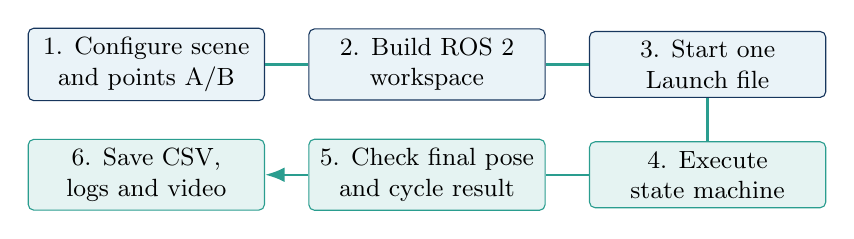
\begin{tikzpicture}[node distance=0.55cm, every node/.style={font=\small}, box/.style={draw=Navy,rounded corners=2pt,fill=Sky,minimum width=3.0cm,minimum height=0.7cm,align=center}, box2/.style={box,draw=Teal,fill=Teal!12}, arr/.style={-Latex,draw=Teal,line width=0.9pt}]
\node[box] (a) {1. Configure scene\\and points A/B};
\node[box,right=of a] (b) {2. Build ROS 2\\workspace};
\node[box,right=of b] (c) {3. Start one\\Launch file};
\node[box2,below=of c] (d) {4. Execute\\state machine};
\node[box2,left=of d] (e) {5. Check final pose\\and cycle result};
\node[box2,left=of e] (f) {6. Save CSV,\\logs and video};
\draw[arr] (a)--(b)--(c)--(d)--(e)--(f);
\end{tikzpicture}
\caption{Experiment workflow from configuration to acceptance evidence.}
\label{fig:workflow}
\end{figure}

\section{Control Principle}
\subsection{Joint-space trajectory generation}
The final configuration uses a set of manually selected joint vectors. For two consecutive waypoints $\mathbf q_0$ and $\mathbf q_1$, the task node uses a cosine interpolation parameter
\[
s(t)=\frac{1-\cos(\pi t/T)}{2},\qquad \mathbf q(t)=\mathbf q_0+s(t)(\mathbf q_1-\mathbf q_0),
\]
where $T$ is the step duration. The zero slope at the two ends reduces abrupt starts and stops. Commands are published at 30 Hz, while each waypoint transition lasts 1.6 s and is followed by a 0.35 s settling interval.

\subsection{State machine and grasp semantics}
The state machine is intentionally explicit: \code{initial}, \code{above\_a}, \code{crab}, \code{pick}, \code{lift}, \code{initial\_2}, \code{release\_ready}, \code{release}, and the final \code{initial}. The gripper opens to 0.12 before approach and uses -0.04 for the final pick version. After the node confirms the grasp, the cylinder is visually attached to the gripper in the Gazebo workflow. At the release point, the node reads the actual target X/Y, moves to a position 0.02 m above that location, opens the gripper, and then fixes the target at $z=0.020$ m. This vertical release avoids a lateral throw and makes the placement check reproducible.

\subsection{Success and safety conditions}
The final object pose is compared with B. A cycle passes when the object is below the configured maximum Z and the XY error is within 0.065 m. The task stops with a failure reason if a waypoint violates a joint limit, a configured fault mode reports an unreachable target or joint-limit fault, a service times out, or the final placement check fails. The final JSON summary records \code{success\_count}, \code{repeat\_count}, the success rule and the failure reason.

\section{Scene and Parameter Configuration}
\begin{table}[H]
\centering\small
\caption{Final fixed-point experiment parameters}
\begin{tabular}{ll}
\toprule
Parameter & Value\\
\midrule
World frame & \code{base}\\
Table size & $0.60\times0.45\times0.04$ m\\
Pick point A & $(0.30,\;0.18,\;0.031)$ m\\
Place point B & $(0.2463,\;-0.1241,\;0.020)$ m\\
Safe height & $0.12$ m\\
Target cylinder & radius $0.018$ m, height $0.050$ m\\
Placement tolerance & XY error $\leq0.065$ m; maximum Z $0.090$ m\\
Control rate / step / settling & 30 Hz / 1.6 s / 0.35 s\\
Repeat count & 5\\
Gripper open / pick & 0.12 / -0.04\\
\bottomrule
\end{tabular}
\end{table}

The green placement area is centered on B. The target cylinder and the support geometry were tuned to radius 0.018 m and 0.020 m, respectively, while the joint trajectory itself was kept unchanged. This is a useful engineering distinction: the geometry was adjusted to match the contact envelope and release area, whereas the taught motion was not silently changed.

\section{ROS 2 Implementation and Operation}
\subsection{Package organization}
The package \code{mecharm\_fixed\_pick\_sim} contains the task node, Launch files, configuration, world and robot description. \code{mycobot\_description} provides meshes and gripper resources. The root script starts the complete experiment and writes logs into \code{logs/fixed\_pick/}. The submission evidence is intentionally outside the source package so that code and results can be reviewed independently.

\subsection{Command-level procedure}
The following commands describe the actual operation record included in the README. They are written as a reproducible sequence rather than as pseudocode.
\begin{enumerate}
\item Source ROS 2 and build the workspace:
\begin{lstlisting}[language=bash]
source /opt/ros/humble/setup.bash
colcon build --symlink-install
source install/local_setup.bash
\end{lstlisting}
\item Start the final five-cycle task with the provided script:
\begin{lstlisting}[language=bash]
./run_contact_grasp.sh
\end{lstlisting}
The script checks for existing Gazebo processes, clears stale overlay variables, sets the Gazebo master URI, and passes \code{repeat\_count:=5}, \code{exit\_on\_complete:=true} and a startup delay to the Launch file.
\item For manual launch, the equivalent ROS 2 command is:
\begin{lstlisting}[language=bash]
ros2 launch mecharm_fixed_pick_sim fixed_point_experiment.launch.py \\
  contact_grasp:=true gui:=true run_task:=true repeat_count:=5 \\
  exit_on_complete:=true task_start_delay_sec:=20.0
\end{lstlisting}
\item Inspect the CSV for \code{grasp\_attached}, \code{released}, \code{release\_settled}, \code{cycle\_passed} and the final JSON summary. The node's topic-level status and the final object pose are both checked; a controller message alone is not treated as proof of placement.
\end{enumerate}

\subsection{ROS 2 interfaces}
The node publishes a state string for the current phase, a result string for terminal status, joint commands for the arm and gripper, and visualization markers for the configured points. The Launch file exposes parameters for GUI mode, task start, repeat count, exit behavior, startup delay and log directory. These parameters allow simulation and hardware runs to share the same control logic while changing only the environment-specific values.

\subsection{Simulation implementation process}
The simulation was implemented as a complete ROS 2 workflow rather than as an isolated Gazebo scene. First, the workspace was sourced and compiled with \code{colcon build --symlink-install}; the local overlay was then sourced so that the Launch system could find both \code{mycobot\_description} and \code{mecharm\_fixed\_pick\_sim}. Second, \code{run\_contact\_grasp.sh} started Gazebo with the contact-mode world, robot description, controllers, robot-state publisher and task node. The script also cleared stale Gazebo environment variables, selected a dedicated master URI and delayed the task until controller activation had completed.

After the scene became stable, the task node executed the same state machine for five repeats. It published interpolated joint commands at 30~Hz, opened the gripper before approaching A, closed it at the pick phase, attached the target cylinder for the simulated grasp, lifted it through the safe height, moved above B, released it vertically and checked the final pose. Each transition was written to CSV with the repeat number, phase, joint positions and status. The simulation process was therefore: build the workspace, launch one controlled Gazebo session, execute the five-cycle state machine, inspect \code{cycle\_passed} rows, and archive the CSV, terminal summary and video.

\subsection{Real-machine implementation process}
The real-machine demonstration reused the motion logic and the semantic phase names established in simulation. Before motion, the physical mechArm 270 was placed beside the prepared tabletop, the gripper was checked in its open state, and the arm was returned to a known home pose. The target and destination were then arranged to match the configured A/B relationship. A short no-load or low-speed check was used to confirm that the arm cleared the table and that the gripper direction was correct before attempting the transfer.

The hardware transfer changes the device-specific communication and controller parameters, while preserving the taught joint waypoints, safe height, gripper commands and release order. During the demonstration the arm approached the target, closed the gripper, lifted and translated to the destination, opened the gripper and returned toward its initial pose. The supplied real-machine MP4 records this physical sequence and is included as visual evidence. Since the archive has no timestamped hardware CSV or separate safety checklist, the video is used to document implementation and operation, while the quantitative five-cycle result in this report remains the verified simulation result.

\section{Verification Results}
\subsection{Five-cycle simulation record}
The two CSV files in the v2 package are distinct SHA-256-verified records. Each contains 116 rows: five complete cycles followed by a terminal summary row. The five \code{cycle\_passed} rows in the recorded run have the following final positions and XY errors.

\begin{table}[H]
\centering\small
\caption{Five-cycle result from \code{fixed\_pick\_20260912\_233915.csv}}
\begin{tabular}{c c c c c}
\toprule
Cycle & $x$ (m) & $y$ (m) & $z$ (m) & XY error (m)\\
\midrule
1 & 0.2457 & -0.1238 & 0.0200 & 0.0006\\
2 & 0.2462 & -0.1241 & 0.0200 & 0.0001\\
3 & 0.2459 & -0.1239 & 0.0200 & 0.0005\\
4 & 0.2466 & -0.1242 & 0.0200 & 0.0003\\
5 & 0.2459 & -0.1239 & 0.0200 & 0.0005\\
\midrule
\multicolumn{4}{r}{Maximum XY error} & 0.0006\\
\bottomrule
\end{tabular}
\end{table}

The terminal row reports \code{success\_count=5}, \code{repeat\_count=5} and the rule “at least 4 successful runs out of 5.” The second CSV gives the same 5/5 result with a maximum XY error of 0.0005 m. The extra repeat value 6 in the CSV is the final summary row emitted after cycle 5; it is not an additional grasp attempt.

\subsection{Static and abnormal-condition checks}
The validation record reports successful Python syntax, Xacro, URDF and \code{colcon build} checks. Before motion, the task node validates each waypoint against the configured joint limits. The error log records the engineering issues encountered while converging to the final version: a simplified gripper collision model could eject the target, an oversized contact envelope could cause penetration, an insufficient startup delay could race controller activation, and a reused release waypoint could create overlapping placements. These cases were resolved by using the contact-mode model, reducing the contact geometry, delaying task start until controllers were ready, and checking the final Gazebo pose after release.

\section{Demonstration Evidence}
\subsection{Simulation video}
Figure~\ref{fig:simvideo} is a three-frame summary extracted from \code{simulation\_demo.webm}. The first frame shows the arm approaching the working area, the middle frame shows the gripper carrying the red cylinder, and the last frame shows the robot back at its initial side of the scene after release. The original WebM is included unchanged in the submission package.
\begin{figure}[H]
\centering
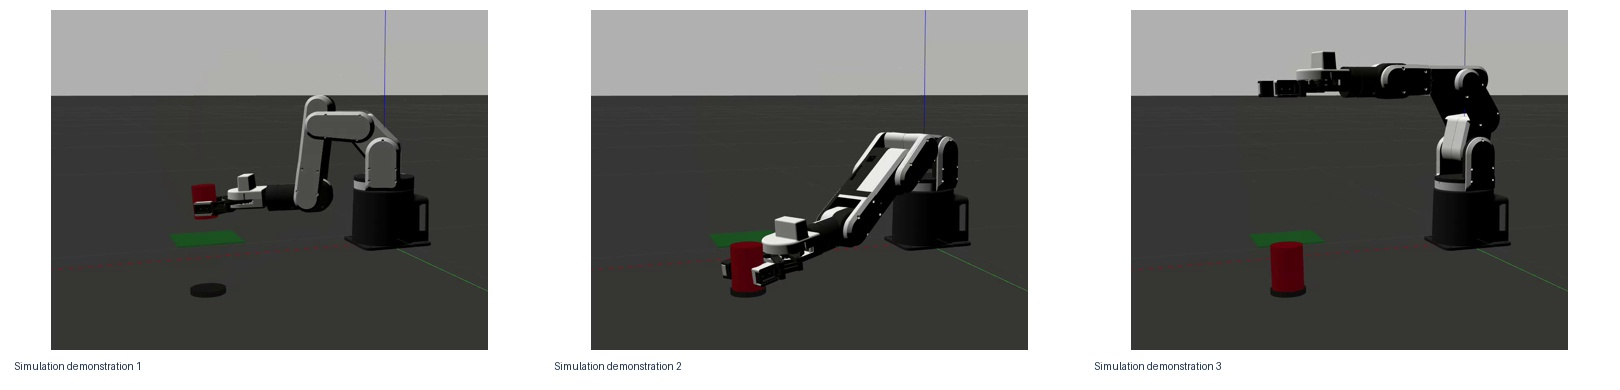
\includegraphics[width=\textwidth]{sim_sequence.jpg}
\caption{Selected frames from the supplied simulation demonstration video.}
\label{fig:simvideo}
\end{figure}

\subsection{Real-machine video}
Figure~\ref{fig:realvideo} summarizes the supplied portrait MP4. It clearly shows the physical arm, gripper, table and target area during operation. It is appropriate evidence that the motion was transferred to hardware. Because the video is not accompanied by a timestamped five-cycle table or a separate safety checklist, the report does not convert the video alone into a numeric success rate.
\begin{figure}[H]
\centering
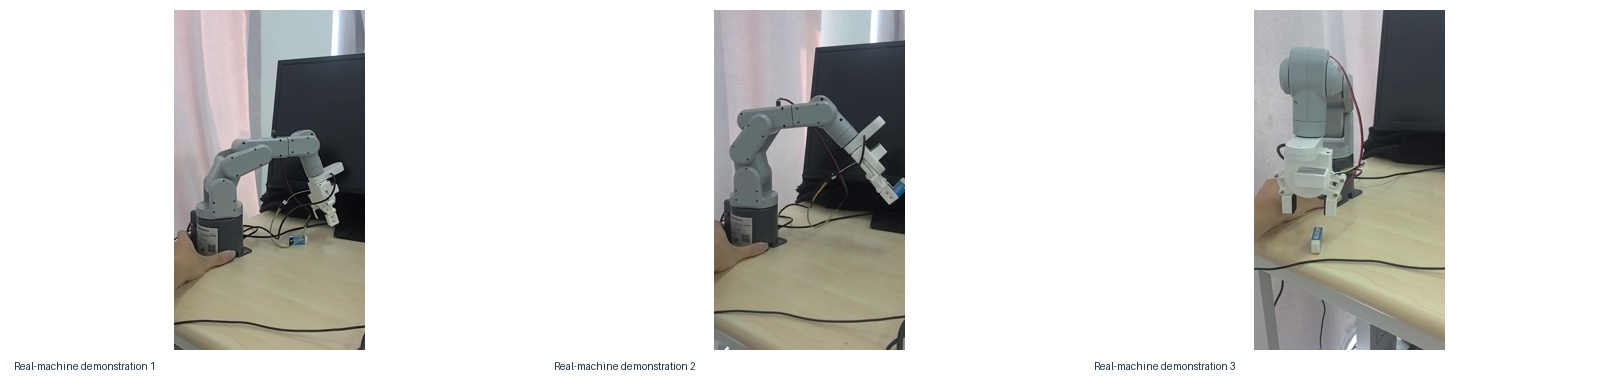
\includegraphics[width=\textwidth]{real_sequence.jpg}
\caption{Selected frames from the supplied real-machine demonstration video.}
\label{fig:realvideo}
\end{figure}

\section{Discussion and Summary}
\subsection{What the experiment demonstrates}
The final simulation package demonstrates a complete fixed-point manipulation loop with explicit parameters, a reproducible state machine, controller startup, object attachment and release semantics, final-pose checking and persistent CSV output. The five-cycle records are stronger than a single successful screenshot because they show repeatability and expose the actual release coordinates. The small maximum XY errors also show that the final vertical-release strategy is consistent with the configured B point.

The source organization makes the experiment easier to reproduce. A new user can build the workspace, run one script, inspect the same named phases, and find the corresponding rows in the log. The separation between source, configuration, evidence and report also supports staged GitHub commits and makes it possible to review changes without downloading a binary archive.

\subsection{Limitations and practical lessons}
The fixed-point task assumes that A and B are known in advance, so it does not solve camera-based localization or dynamic obstacle avoidance. The Gazebo visual attachment workflow is deliberately controlled to make grasp and release measurable; a physical gripper has additional effects such as compliance, friction variation, cable interference and object slip. The supplied real-machine video therefore complements, but does not replace, a numeric hardware test record.

The debugging history shows why final-pose verification matters. A node can report that a gripper closed or that an object was visually attached while the physical or simulated object still ends outside the target area. Checking the object's final X/Y/Z, recording the release-above and release-settled events, and preserving the error log turns a visually plausible demo into a traceable experiment.

\subsection{Summary and reflection}
\begin{enumerate}
\item A fixed-point manipulation task is primarily a consistency problem: coordinate frames, taught joint vectors, gripper values, object geometry and success thresholds must describe the same scene.
\item A state machine with explicit phases is easier to diagnose than a long unlabelled command stream. The phase names in the CSV make it possible to locate the first failed action.
\item Safe operation requires checks before motion and after release. Joint-limit validation prevents invalid commands, while final-pose checking prevents false positives.
\item ROS 2 Launch and parameter files provide the bridge from simulation to hardware. The control sequence can remain stable while device and environment parameters change.
\item The final deliverable is more useful when it contains source, logs, videos, report source and PDF together, with checksums for the evidence files and a staged Git history that records how the package was assembled.
\end{enumerate}

\section{Submission File Map}
\begin{table}[H]
\centering\small
\caption{Files included in the final submission directory}
\begin{tabularx}{\textwidth}{>{\ttfamily\footnotesize}p{0.39\textwidth}X}
\toprule
Path & Purpose\\
\midrule
\code{src/mecharm\_fixed\_pick\_sim/} & ROS 2 task node, Launch, YAML, world and URDF/Xacro\\
\code{src/mycobot\_description/} & Robot meshes and gripper description resources\\
\code{run\_contact\_grasp.sh} & One-command five-cycle simulation launch\\
\code{submission\_evidence/results/} & Two independent five-cycle CSV records\\
\code{submission\_evidence/docs/ERROR\_LOG.md} & Abnormal cases and fixes\\
\code{submission\_evidence/videos/} & Simulation WebM and real-machine MP4\\
\code{submission\_evidence/SHA256SUMS.txt} & Hashes for the evidence files\\
\code{report/experiment2\_lab\_report.tex} & This report source\\
\code{report/experiment2\_lab\_report.pdf} & Compiled report for submission\\
\bottomrule
\end{tabularx}
\end{table}

\subsection{GitHub commit record}
The experiment-two materials are maintained in the dedicated public repository
\url{https://github.com/9161942-boop/robotics-experiment-2}. The upload was split into four commits so that the code, evidence, report and videos can be reviewed independently:
\begin{table}[H]
\centering\small
\caption{Staged GitHub commits for Experiment 2}
\begin{tabular}{ll}
\toprule
Commit & Content\\
\midrule
\code{b21bb71} & ROS 2 packages, Launch files and simulation configuration\\
\code{330ac6a} & Five-cycle CSV records, error log and checksums\\
\code{dc85c53} & English LaTeX report, PDF and figures\\
\code{b4f67d2} & Simulation and real-machine demonstration videos\\
\bottomrule
\end{tabular}
\end{table}

\section*{Declaration of Evidence Scope}
\addcontentsline{toc}{section}{Declaration of Evidence Scope}
The simulation results in this report are quoted from the supplied final v2 archive and its CSV/validation records; no new simulation was run while preparing this report. The two videos are the user-supplied demonstration files and were inspected read-only. Statements about the exact five-cycle simulation count are supported by the CSV files. Statements about the real-machine demonstration are limited to what is visible in the supplied MP4 unless a separate hardware result table is added later.

\begin{center}
\small\textbf{Figure 4.} GitHub commit history for the public Experiment 2 repository\\[2pt]
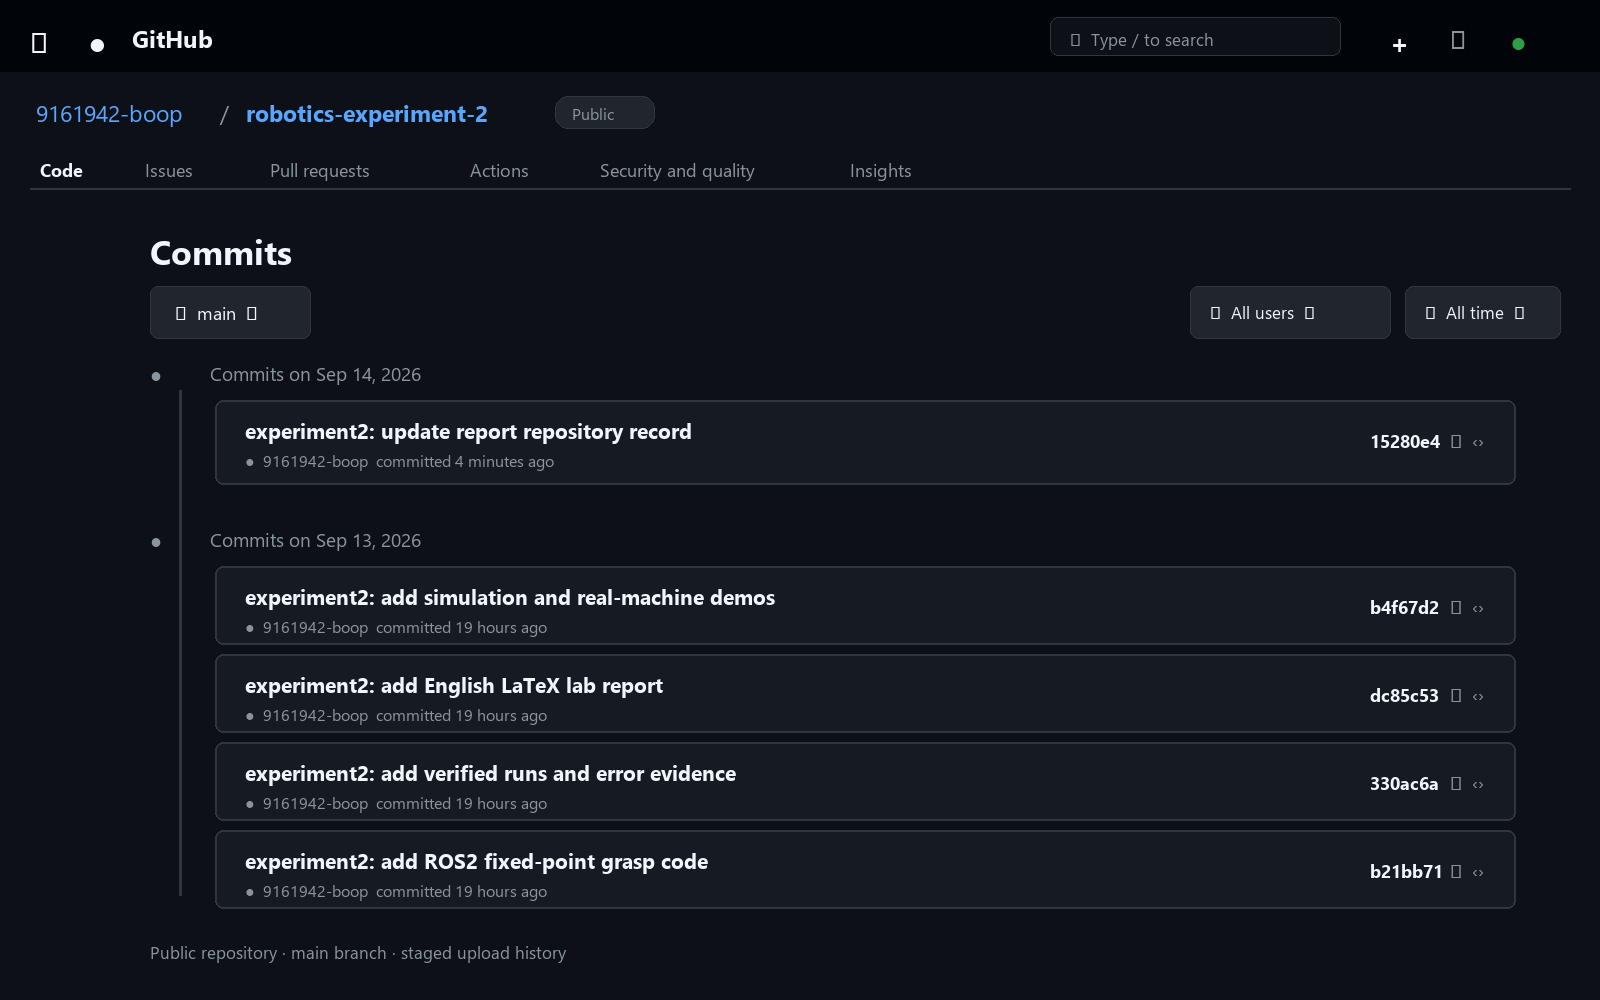
\includegraphics[width=0.55\textwidth]{github_commit_history_exp2.png}
\label{fig:github-history}
\end{center}

\end{document}
